\chapter{Controlador de corriente} \chapterlabel{Informe/4-ControladorCorriente} \label{cap:ControladorCorriente}

En este capítulo se diseña y modela el circuito encargado de controlar la corriente que circula por el electroimán. Como se vio en el capítulo anterior, el sistema trabaja con corrientes elevadas por lo que se implementan estrategias de conmutación para reducir las pérdidas de energía. Para ello se utiliza una topología de puente H con cuatro MOSFET y un \textsl{driver} que los controla. Además, se detallan los criterios tenidos en cuenta al momento de  elegir  y dimensionar todos los componentes que intervienen para lograr el correcto funcionamiento del controlador de corriente. Por último, se obtiene su función transferencia  para ser utilizada en el diseño del compensador.

\section{Descripción general}\label{sec_descripcion-general}

Para mantener en suspensión a la pieza móvil es necesario regular la fuerza electromagnética que genera el electroimán según sea necesario. Como se analizó en el capitulo \ref{cap:CaracterizacionElectroiman}, en la sección ASDASDAS se llega a la ecuación \ref{eq_fuerza_magnetica}, que se repite a continuación. 

\begin{equation*}
	\abs{F_{m}}=\frac{i^{2}*N^{2}*\mu_{o}*A}{4*Y_{g}^{2}}
\end{equation*}

En ella se ve que la fuerza magnética depende de la corriente del bobinado. Por lo tanto si se desea regular la fuerza electromagnética, se puede lograr a partir de modificar la intensidad de corriente.

\colorbox{red}{esto estaba antes}}Esto se logra modificando la intensidad de la corriente que circula por su bobinado como lo indica la expresión \ref{eq_fuerza_magnetica}. Por lo tanto, es necesario diseñar una fuente de alimentación que sea capaz de proveer la corriente requerida. 

\subsection{Análisis de respuesta al escalón}

Como se analizó en el capítulo \ref{cap:CaracterizacionElectroiman}, el electroimán puede ser modelado como una inductancia que varía con la distancia de entrehierro y una resistencia serie. Es decir, como un circuito RL serie cuya admitancia se muestra en la expresión \ref{eq_corriente}.

\begin{equation} \label{eq_corriente}
\frac{I_L}{V_L}(s)=\frac{1}{sL(Y_g)\ +\ R_L}
\end{equation}

Al aplicar la transformada inversa de Laplace a la expresión  \ref{eq_corriente}, se obtiene la respuesta temporal de la corriente ante un escalón de tensión con amplitud $v_L$ en la entrada, considerando corriente inicial $I_o$ y constante de tiempo $\tau=\frac{L(Y_g)}{R_L}$.

\begin{equation} \label{eq_corriente_temporal_cond_iniciales}
	i_L(t)=\frac{v_L}{R_L} + (I_o-\frac{v_L}{R_L})*e^{-\frac{t}{\tau}}
\end{equation}

En la expresión \ref{eq_corriente_temporal_cond_iniciales} se puede observar que la respuesta al escalón está compuesta por dos partes: un término con una exponencial negativa correspondiente al transitorio, y un término constante correspondiente al valor en régimen permanente $\frac{v_L}{R_L}$. El primero es el responsable de que la corriente en el inductor crezca de manera amortiguada, hasta alcanzar el valor de régimen permanente luego de cierto tiempo. Este comportamiento se puede observar en la simulación realizada en la figura \ref{fig:img_respuesta_escalon}. En la parte superior se observa la tensión de entrada y, en la inferior, la corriente del electroimán. Este análisis resulta de utilidad para conocer el comportamiento del electroimán y diseñar un controlador de corriente adecuado.


\begin{figure}[H]
	\centering
	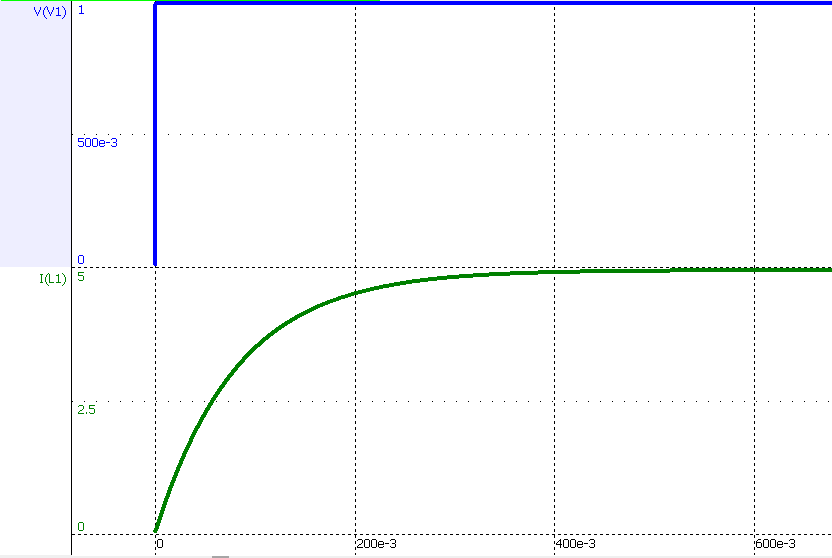
\includegraphics[scale=0.5]{corriente_escalon.png}
	\caption{Respuesta ante una entrada en escalón.}
	\label{fig:img_respuesta_escalon}
\end{figure}


\section{Diseño del controlador}




----------------------------------------

Se desea lograr controlar el valor medio de corriente que circula por el electroimán a partir de un sistema realimentado. Para ello se propone utilizar un controlador que trabaja en conmutación, alternando la alimentación del electroimán entre un valor superior positivo $\ V_{sup}$, y un valor inferior negativo $V_{inf}$. De esta manera, al controlar los tiempos de conmutación, se puede lograr una forma de onda como la que se muestra en la figura  \ref{fig:img_corriente_exponencial}. El resultado es que se obtiene una forma de onda oscilante cuyo valor medio $<I_L>$ es la corriente deseada. El resultado es una forma de onda con un valor medio correspondiente al deseado y un ripple superpuesto. La idea es que este ripple sea pequeño comparado con el valor medio, de manera que la planta pueda filtrarlo. 

\begin{figure}[H]
	\centering
	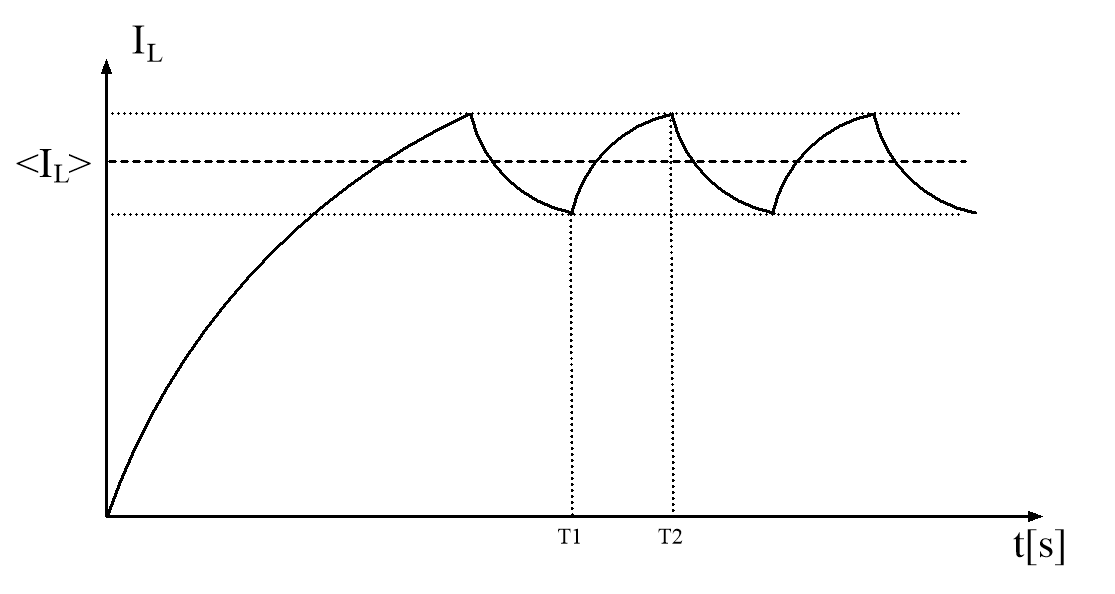
\includegraphics[scale=0.5]{Forma-de-onda-corriente-exponencial.png}
	\caption{Forma de onda de corriente y tensión en el electroimán.}
	\label{fig:img_corriente_exponencial}
\end{figure}

\colorbox{red}{modificar valores de imagen}

Si se elige un período de conmutación lo suficientemente chico con respecto a la constante de tiempo de la planta, la forma de onda de la corriente en estado estacionario puede ser aproximada a una onda triangular como se muestra en la figura daddasdas.

\begin{figure}[H]
	\centering
	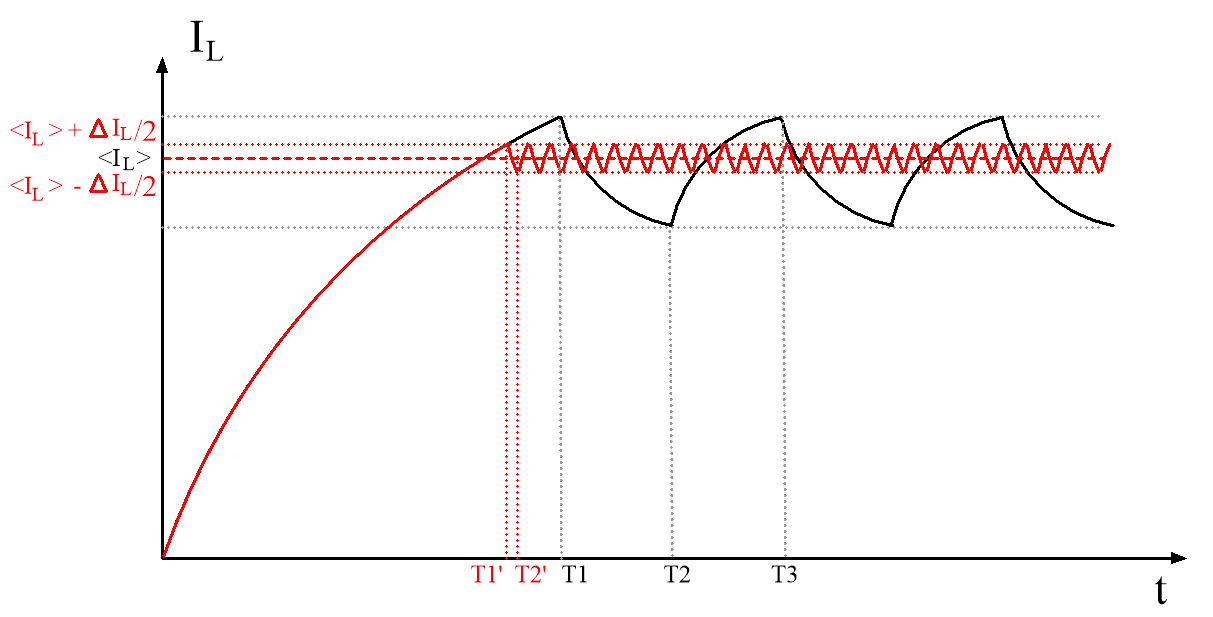
\includegraphics[scale=0.5]{Forma-de-onda-corriente-lineal.png}
	\caption{Forma de onda de corriente al disminuir el período de conmutación.}
	\label{fig:img_corriente_lineal}
\end{figure}

Se puede obtener una expresión lineal para cada tramo de la corriente triangular a partir de la serie de Taylor hasta el término de orden 1 de la ecuación \ref{eq_corriente_temporal_cond_iniciales}:

\begin{equation} \label{eq_corriente_taylor}
	i_L(t)=I_o -  (I_o-\frac{v_L}{R_L})*\frac{t}{\tau}
\end{equation}

Por el momento se considera el caso en que $I_o=0$, y considerando que $\tau=\frac{L}{R_L}$, de manera que la expresión queda:

\begin{equation} \label{eq_corriente_taylor_2}
	i_L(t)= \frac{v_L}{L}*t
\end{equation}

De ACA se puede obtener la pendiente como:

\begin{equation} \label{eq_corriente_taylor_2}
	\frac{di_L(t)}{dt}= \frac{v_L}{L}
\end{equation}


Como se vió en el capítulo 2, la inductancia es inversamente proporcional a la distancia de entrehierro, por lo tanto resulta:

\begin{equation} \label{eq_corriente_taylor_2}
	\frac{di_L(t)}{dt}= v_L*f(Y_g)
\end{equation}

Utilizando la expresión \ref{eq_inductancia_vs_y}, se llega a:

\begin{equation} \label{eq_corriente_taylor_2}
	\frac{di_L(t)}{dt}= Y_g*\frac{2}{N^2*A*\mu_o}*v_L
\end{equation}

Mirando la imagen 3.3 se puede plantear dos casos para la pendiente: la de subida, cuando $v_L=V_{sup}$ y la de bajada cuando $v_L=V_{inf}$ se obtienen dos expresiones para la pendiente:

\begin{equation} \label{eq_corriente_taylor_2}
	\frac{di_L(t)}{dt}_{sup}= Y_g*\frac{2}{N^2*A*\mu_o}*V_{sup}
\end{equation}


\begin{equation} \label{eq_corriente_taylor_2}
	\frac{di_L(t)}{dt}_{inf}= Y_g*\frac{2}{N^2*A*\mu_o}*V_{inf}
\end{equation}



Se puede observar que la pendiente está compuesta en su mayoría por constantes... Por lo tanto, si se elige que $|V_{sup}|=|V_{inf}|=|V_{cc}|$, la pendiente queda dependiendo únicamente de la distancia $Y_g$ como se muestra en la ecuación de ABAJO:

\begin{equation} \label{eq_corriente_taylor_2}
	\frac{di_L(t)}{dt}= Y_g*\frac{2}{N^2*A*\mu_o}*V_{cc}
\end{equation}


Este análisis resulta de interés ya que se puede observar que la pendiente tiene información de la distancia de entrehierro. Por lo tanto, se podría aplicar un estimador de posición a partir de medir la pendiente.

 se podría aprovechar esa relación para aplicar estimación de variables y obtener, de manera indirecta un valor de distancia de entrehierro a partir de la pendiente de la corriente de la onda de corriente conmutada.

Como se mencionó en la descripción general del dispositivo, es de interés realizar una estimación de la distancia del entrehierro a partir de la corriente que circular en el electroimán. Por este motivo es conveniente aprovechar la relación que existe entre la pendiente de la onda triangular, con la inductancia, que es inversamente propocional a la distancia de entrehierro.... De esta manera se puede implementar un circuito de estimación que trabaje a partir de medir la pendiente... Paroa que este circuito funcione correctamente, se debe respetar dos condiciones:

*Que la magnitud de la pendiente solo sea sensible a la distancia de separación, y que todo lo demás sea constante (v_L)...

*Que la pendiente en la subida sea igual en valor absoluto a la de bajada.  PAra que se pueda obtener un valor de posición en todo momento, sin que el sistema quede a lazo abierto

*Que la estimación nunca se vea interrumpida, ya que el sisema quedaría a lazo abierto.
